\subsection{Cost Category 70: Annualized O\&M Cost (AOC)}

The Operations and Maintenance (O\&M) costs was previously estimated to be 2 \% of the direct cost, assessed annually.  The O\&M cost depends on the system complexity and the requirements of regulations, security and maintenance. The costs are computed based on look-up tables, such as the one shown in Fig. \ref{fig:statista} at 60 USD per kilowatt-year.  

\begin{figure}[b!] 
\centering 
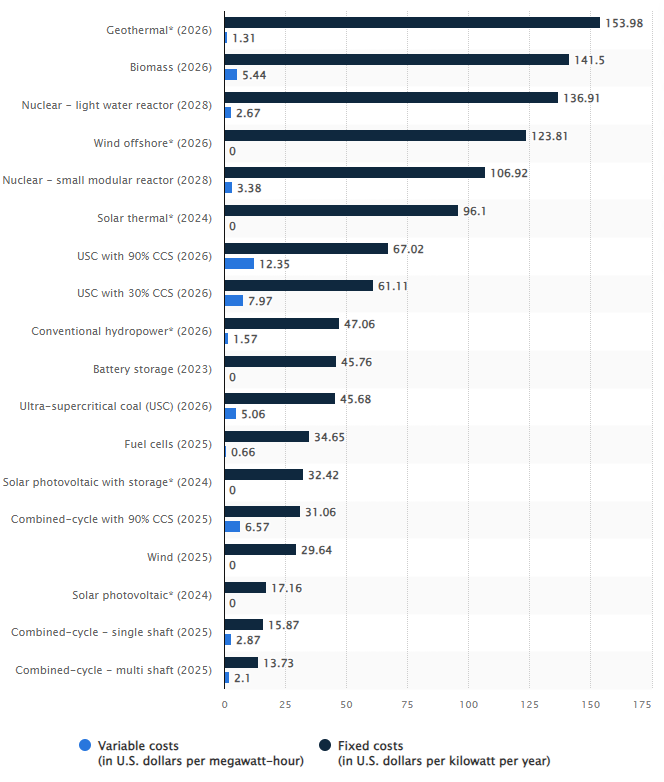
\includegraphics[scale=0.5]{StandardFigures/statista.png} 
\caption{Operations and Maintenance costs for various kinds of power plants.} 
\label{fig:statista} 
\end{figure} 

\begin{verbatim} 
C_OM = 60 * PE * 1000 = 62  
\end{verbatim} 

Annualized O\&M costs are \$ 62 M.

\subsubsection*{Cost Category 71 – O\&M Staff}
Component in the financial structuring of operational expenditures in various industries, especially those involving significant infrastructure and machinery, such as power generation, manufacturing, and utilities.  The costs under Cost Category 71 predominantly include:

\begin{itemize}
    \item \textbf{Salaries:} The regular wages paid to the O\&M staff.
    \item \textbf{Training and Development:} Costs associated with professional development, training programs, and certifications to ensure staff is up-to-date with the latest operational and maintenance practices.
    \item \textbf{Overtime and Shift Allowances:} Compensation for extended work hours and shift differentials, especially in 24/7 operational setups.
\end{itemize}

Cost Category 71 is crucial in operational budgeting due to:

\begin{enumerate}
    \item \textbf{Staffing Optimization:} The need for an optimal number of skilled staff to ensure efficient and safe operations.
    \item \textbf{Direct Impact on Operational Efficiency:} The performance and availability of O\&M staff directly affect operational uptime and efficiency.
    \item \textbf{Regulatory Compliance:} Compliance with labor laws and industry-specific regulations regarding staffing and worker safety.
\end{enumerate}

\textit{Cost Category 71 – O\&M Staff} encompasses all aspects of costs related to the personnel responsible for the operation and maintenance of facilities. Efficient management of this category is vital for ensuring operational excellence, staff well-being, and overall financial health of the organization.


\subsubsection*{Cost Category 72 – Management Staff}
Crucial aspect of operational expenses in various sectors, especially in industries where effective management plays a pivotal role in ensuring efficient operations and achieving organizational objectives.  Cost Category 72 typically encompasses:

\begin{itemize}
    \item \textbf{Salaries:} The basic remuneration paid to operations management staff.
    \item \textbf{Bonuses and Incentives:} Performance-related bonuses and incentives that align management objectives with corporate goals.
    \item \textbf{Professional Development:} Expenses related to the continuous learning and development of management skills, including workshops, seminars, and courses.
    \item \textbf{Leadership Training:} Specific training focused on enhancing leadership qualities necessary for effective management.
\end{itemize}

The inclusion of Cost Category 72 in operational expenditure is significant due to:

\begin{enumerate}
    \item \textbf{Strategic Decision Making:} Management staff play a crucial role in strategic decision-making and operational planning.
    \item \textbf{Operational Efficiency:} Effective management is key to ensuring operational efficiency and organizational success.
    \item \textbf{Staff Leadership:} Management staff are responsible for leading, guiding, and motivating the workforce, directly impacting productivity and morale.
\end{enumerate}

\subsubsection*{Cost Category 73 – Salary-Related Costs}
This Cost Category includes taxes, insurance, fringes, benefits, and any other annual salary-related costs.

\subsubsection*{Cost Category 74 – Operations Chemicals, and Lubricants}

\subsubsection*{Cost Category 75 – Spare Parts}
Critical element in the operational budgeting of various industries, particularly in sectors that rely on continuous and efficient machinery and equipment operation.  This cost category encompasses:

\begin{itemize}
    \item \textbf{Operational Spare Parts:} Expenses associated with spare parts used in regular operations. These do not include major equipment or capital plant upgrades.
    \item \textbf{Exclusion of Capitalized Items:} It specifically excludes items that would be capitalized or amortized over a period or quantity of product.
\end{itemize}

Cost Category 75 plays a significant role in Operations and Maintenance (O\&M) budgeting, as it:

\begin{itemize}
    \item \textbf{Ensures Operational Continuity:} Regular replacement and availability of spare parts are crucial for uninterrupted operations.
    \item \textbf{Impacts Maintenance Scheduling:} Influences the planning and scheduling of maintenance activities.
    \item \textbf{Affects Operational Efficiency:} Directly impacts the overall efficiency and lifespan of the operational equipment.
\end{itemize}

\textit{Cost Category 75 – Spare Parts} is essential for the smooth operation and maintenance of machinery and equipment in various industries. It encompasses the costs of spare parts necessary for regular operation and scheduled component replacements, playing a vital role in operational budgeting and efficiency.  Cost of any operational spare parts, excluding capital plant upgrades or major equipment that will be capitalized or amortized over some period or quantity of product.

\subsubsection*{Cost Category 76 – Utilities, Supplies, and Consumables}
Cost of water, gas, electricity, tools, machinery, maintenance equipment, office supplies and similar items purchased annually.

\subsubsection*{Cost Category 77 – Capital Plant Upgrades}
Upgrades to maintain or improve plant capacity, meet future regulatory requirements or plant life extensions.

\subsubsection*{Cost Category 78 – Taxes and Insurance}
Property taxes and insurance costs, excluding salary related.

\subsubsection*{Cost Category 79 – Contingency on Annualized O\&M Costs}
This Cost Category includes an assessment of additional cost necessary to achieve the desired confidence level for the annualized O\&M costs not to be exceeded.
